\documentclass[11pt]{article}

\usepackage{spikey}
\usepackage{amssymb}
\usepackage{float}
\usepackage[margin=1in]{geometry}

\usepackage{setspace}
\linespread{1.5}


\title{Probabilistic Graphical Models}
\author{Tianyu Du}

\newcommand{\dsep}[0]{\text{d-sep}}
\newcommand{\sep}[0]{\text{sep}}
\newcommand{\pa}[0]{\text{Par}}

\begin{document}
	\maketitle
	\section{Graphical Representations}
	\subsection{Factors}
	\begin{definition}
		Let $X_1, X_2, \cdots, X_k$ be a set of random variables, then a \textbf{factor} $\phi$ is a mapping from values of these random variables to $\R$.
		\begin{align}
			\phi: Val(X_1, X_2, \cdots, X_k) \to \R
		\end{align}
		The set of random variables $\{X_1, X_2, \cdots, X_k\}$ is defined as the \textbf{scope} of $\phi$.
	\end{definition}
	
	\begin{remark}
		In principle, a factor can take any value in $\R$. However, in practice, we restrict our considerations to factors with positive ranges only.
	\end{remark}
	
	\begin{definition}
		Let $\phi_1$ and $\phi_2$ be two factors with scopes $\{A,B\}$ and $\{B, C\}$.
		Then the \textbf{factor product} $\phi_1 \times \phi_2$ is a factor with scope $\{A, B, C\}$ defined as
		\begin{align}
			\phi_1 \cdot \phi_2 (a, b, c) = \phi_1(a, b) \cdot \phi_2(b, c)
		\end{align}
	\end{definition}
	
	\begin{definition}
		Let $\phi$ be a factor with scope $\{A, B, C\}$, then \textbf{marginalizing $C$ from $\phi$} results in a factor $\phi'$ with scope $\{A, B\}$ defined as the following:
		\begin{align}
			\phi'(a, b) = \sum_{c \in Val(C)} \phi(a, b, c)
		\end{align}
	\end{definition}
	
	\begin{definition}
		The \textbf{factor reduction} operation restricts $\phi(A,B,C)$ to take only a specific value of $C=c$, and results in a factor $\phi'$ with scope $\{A, B\}$.
		\begin{align}
			\phi'(a, b) = \phi(a, b, c)
		\end{align}
	\end{definition}
	
	\subsection{Semantics and Factorization}
	\begin{definition}
		A \textbf{Bayesian network} consists of (i) a directed acyclic graph (DAG) $G$ whose nodes correspond to random variables $X_1, \cdots, X_n$
		 (ii) and a conditional probability distribution $P(X_i|Par_G(X_i))$ for each node $X_i$. The joint distribution is defined as the factorization
		 \begin{align}
		 	P(X_1, \cdots, X_n) &= \prod_{i=1}^n P(X_i|\pa_G(X_i))
		 \end{align}
	\end{definition}
	
	\begin{definition}
		Let $G$ be a graph over $X_1, \cdots, X_n$, then the joint probability $P$ \textbf{factorizes} over $G$ if and only if
		\begin{align}
			P(X_1, \cdots, X_n) &= \prod_{i=1}^n P(X_i|\pa_G(X_i))
		\end{align}
	\end{definition}
	
	\subsection{Pass of Influences in Bayesian Networks}
	\begin{definition}
		A path $X_1 - \dots - X_k$ in Bayesian network $G$ is \textbf{active} if there is no explaining-away structure $X_{i-1} \rightarrow X_i \leftarrow X_{i+1}$ in it.
	\end{definition}
	
	\begin{definition}
		Let $Z \subseteq V_G$ be a set of random variables in the Bayesian network, then a path $X_1 - \dots - X_k$ in $G$ is \textbf{active conditioned on $Z$} if 
		\begin{enumerate}
			\item for all explaining-away structure $X_{i-1} \rightarrow X_i \leftarrow X_{i+1}$ in the path, $X_i$ or some decedents of $X_i$ are in $Z$,
			\item \ul{and} no other node in the path is in $Z$.
		\end{enumerate}
	\end{definition}
	
	\begin{definition}
		Let $X, Y, Z \subseteq V_G$, if there is no path from $X$ to $Y$ is active conditioned on $Z$, then $X$ and $Y$ are \textbf{d-separated} by $Z$ in graph $G$ denoted as $\dsep_G(X, Y|Z)$.
	\end{definition}
	
	\subsection{Independencies and Factorizations}
	\begin{definition}
		Let $X, Y, Z$ be random variables with distribution $P$, then $X \indep Y$ if and only if $P(X, Y) = P(X)P(Y)$, $X \indep Y | Z$ if and only if $P(X, Y|Z) = P(X|Z)P(Y|Z)$.
	\end{definition}
	
	\begin{proposition}
		Let $X, Y, Z$ be random variables with distribution $P$, then $X \indep Y$ if and only if $P(X,Y)$ factorizes as the following
		\begin{align}
			P(X, Y) \propto \phi_1(X) \phi_1(Y) \label{eq:1}
		\end{align}
		and $X \indep Y|Z$ if and only if $P(X, Y, Z)$ factorizes as
		\begin{align}
			P(X, Y, Z) \propto \phi_1(X, Z) \phi_1(Y, Z) \label{eq:2}
		\end{align}
		
		\begin{proof}
			Relation (\ref{eq:1}) follows the definition immediately.
			Suppose $X \indep Y|Z$, then
			\begin{align}
				P(X, Y | Z) &= P(X|Z)P(Y|Z) \\
				\iff P(X,Y,Z) &= P(X|Z)P(Y|Z)P(Z) \\
				P(X,Y,Z) &\propto P(X|Z)P(Z)P(Y|Z)P(Z) \\
				&= P(X,Z) P(Y,Z) \\
				&= \phi_1(X, Z) \phi_1(Y, Z)
			\end{align}
		\end{proof}
	\end{proposition}
	
%	\begin{proposition}
%		Generally, let $P$ be a distribution on random variables $X_1, \cdots, X_n$, then $X_i \indep X_j$ if and only if the factorization of $P$ contains $\phi_i(X_i)$ and $\phi_j(X_j)$.
%	\end{proposition}
	
	\begin{theorem}[Factorization$\implies$Independence]
		If $P$ factorizes over $G$, and $\dsep_G(X,Y|Z)$ then $P$ satisfies $(X\indep Y|Z)$.
%		\begin{proof}
%			Let $V$ denote the set of all random variables in the network and $V \backslash \{X, Y, Z\} = \{V_1, V_2, \cdots, V_n\}$.
%			Because $P$ factorizes over $G$,
%			\begin{align}
%				P(X, Y, Z) &= \sum_{V_i: i=1,\cdots, n} P(X, Y, Z, V_1, V_2, \cdots, V_n) \\
%				 &=\sum_{V_i: i=1,\cdots, n} P(X|\pa_G(X)) P(Y|\pa_G(Y)) P(Z|\pa_G(Z)) \prod_{i=1}^n P(V_i|\pa_G(V_i))
%			\end{align}
%		\end{proof}
	\end{theorem}
	
	\begin{theorem}[Causal Markov Condition]
		For any random variable $X_i$ in the Bayesian network, $X_i$ is d-separated from all its non-descendants by $\pa_G(X_i)$.
	\end{theorem}
	
	\begin{corollary}
		If $P$ factorizes over $G$, then in $P$, any variable is independent of its non-descendants given its parents.
	\end{corollary}
	
	\begin{definition}
		Let $\mc{I}(G)$ denote the collection of independencies implicitly encoded by d-separations in graph $G$,
		\begin{align}
			\mc{I}(G) := \{(X\indep Y|Z): X, Y, Z \in V\ s.t.\ \dsep_G (X, Y | Z)\}
		\end{align}
		If a distribution $P$ over $V$ satisfies all independencies in $\mc{I}(G)$, then we say that $G$ is an \textbf{I-map} (independency map) of $P$.
		
		That is, the I-map of distribution $P$ is a graphical representation of all (and probably more) independencies of $P$.
	\end{definition}
	
	\begin{example}
		Let $P$ be a probability distribution and let $G$ be an I-map for $P$. Let $\mc{I}(P)$ and $\mc{I}(G)$ denote sets of independencies in $P$ and $G$.
		Suppose $G$ is a I-map of $P$, then all independencies encoded in $G$ are satisfied by $P$, therefore,
		\begin{align}
			\mc{I}(G) \subseteq \mc{I}(P)
		\end{align}
	\end{example}
	
	\begin{example}
		The I-map can be used for two graphs as well. $G_1$ is a I-map of $G_1$ if $\mc{I}(G_1) \subseteq \mc{I}(G_2)$.
		That is, $G_1$ is an I-map of $G_2$ if it does not make independence assumptions that are not true in $G_2$.
	\end{example}
	
	\begin{theorem}[Independence$\implies$Factorization]
		If $G$ is an I-map for $P$, that is, $P$ adheres all independencies encoded in $G$, then $P$ factorizes over $G$.
%		\begin{proof}
%			
%		\end{proof}
	\end{theorem}
	\subsection{Template Models}
	\begin{definition}
		A \textbf{template variable} $X(U_1, \cdots, U_k)$ is instantiated (duplicated) multiple times in a graph.
		\textbf{Template models} are languages that specify how ground variables (i.e., instantiations of template variables) inherit dependency model from template.
	\end{definition}
	
	\begin{notation}
		Let $X^{(t)}$ denote the variable at time $t \Delta$, where $\Delta$ is the time granularity in the discrete timeline.
		Let $X^{(t:t')} = \{X^{(t)}, ^{(t+1)}, \cdots, X^{(t')}\}$ denote the set of variables over a period of time.
	\end{notation}
	
	\begin{definition}
		A Bayesian network is said to satisfy the \textbf{Markov assumption} if
		\begin{align}
			X^{(t+1)} \indep X^{(0:t-1)} | X^{(t)}
		\end{align}
		When Markov assumption holds, we may express the joint distribution of all $X$ as
		\begin{align}
			P(X^{(0:T)}) = P(X^{(0)}) \prod_{t=0}^{T-1} P(X^{(t+1)}|X^{(t)})
		\end{align}
	\end{definition}
	
	\begin{definition}
		A series of random variables $X^{(0)}, X^{(1)}, \cdots, X^{(T)}$ satisfies the \textbf{time invariance} assumption if there exists a template probability model $P(X'|X)$ such that for all $t$,
		\begin{align}
			P(X^{(t+1)}|X^{(t)}) = P(X'|X)
		\end{align}
	\end{definition}
	
	\begin{definition}
		A \textbf{2-time-slice Bayesian network} (2TNB) over $X_1, \cdots, X_n$ (that is, $n$ random variables for each time step) is specified as a Bayesian network fragment such that
		\begin{itemize}
			\item The nodes include $X_1', \cdots, X_n'$ and a subset of $X_1, \cdots, X_n$,
			\item and only the nodes $X_n', \cdots, X_n'$ have parents and a conditional probability distribution.
		\end{itemize}
		Further, the 2TBN defines a conditional distribution
		\begin{align}
			P(X'|X) = \prod_{i=1}^n P(X_i' | \pa(X_i'))
		\end{align}
	\end{definition}
	
	\begin{definition}
		A \textbf{dynamic Bayesian network} (DNB) over $X_1, \cdots, X_n$ is defined by
		\begin{itemize}
			\item a 2TNB, BN$_{\rightarrow}$, over $X_1, \cdots, X_n$,
			\item and a Bayesian network, BN$^{(0)}$, over $X_1^{(0)}, \cdots, X_n^{(0)}$.
		\end{itemize}
	\end{definition}
	
	\begin{definition}
		For a trajectory over $0, \cdots, T$, the \textbf{ground (unrolled) network} of a DNB is a model such that
		\begin{itemize}
			\item the dependency model for $X_1^{(0)}, \cdots, X_n^{(0)}$ is copied from BN$^{(0)}$,
			\item and the dependency model for $X_1^{(t)}, \cdots, X_n^{(t)}$ is copied from BN$_{\rightarrow}$.
		\end{itemize}
	\end{definition}
	
	\subsection{Plate Models}
	\par We can use plate models to represent repetitions.
	\begin{example}
		Let $O_t \overset{i.i.d.}{\sim} \tx{Bernoulli}(\theta)$, and $\{O_t\}_t$ is simply a set of coin tosses outcomes. Such scenario can be modelled as in Figure \ref{fig:1.2.4.1}. Figure \ref{fig:1.2.4.2} illustrates an equivalent representation of this plate model.
	\end{example}

	\begin{figure}[H]
		\caption{A plate model for Bernoulli trails}
		\centering
		\medbreak
		\label{fig:1.2.4.1}
		\tikzset{every picture/.style={line width=0.75pt}} %set default line width to 0.75pt        
		
		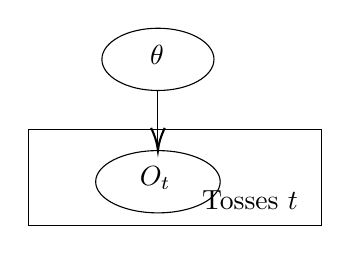
\begin{tikzpicture}[x=0.75pt,y=0.75pt,yscale=-1,xscale=1]
		%uncomment if require: \path (0,300); %set diagram left start at 0, and has height of 300
		
		%Shape: Rectangle [id:dp9459242100341441] 
		\draw   (158.51,104) -- (300,104) -- (300,150) -- (158.51,150) -- cycle ;
		%Straight Lines [id:da7972474226847348] 
		\draw    (221,85) -- (221,111.96) ;
		\draw [shift={(221,113.96)}, rotate = 270] [color={rgb, 255:red, 0; green, 0; blue, 0 }  ][line width=0.75]    (10.93,-3.29) .. controls (6.95,-1.4) and (3.31,-0.3) .. (0,0) .. controls (3.31,0.3) and (6.95,1.4) .. (10.93,3.29)   ;
		%Shape: Ellipse [id:dp0226909827079409] 
		\draw   (194,70) .. controls (194,61.72) and (206.09,55) .. (221,55) .. controls (235.91,55) and (248,61.72) .. (248,70) .. controls (248,78.28) and (235.91,85) .. (221,85) .. controls (206.09,85) and (194,78.28) .. (194,70) -- cycle ;
		%Shape: Ellipse [id:dp597261072710862] 
		\draw   (191,128.96) .. controls (191,120.67) and (204.43,113.96) .. (221,113.96) .. controls (237.57,113.96) and (251,120.67) .. (251,128.96) .. controls (251,137.24) and (237.57,143.96) .. (221,143.96) .. controls (204.43,143.96) and (191,137.24) .. (191,128.96) -- cycle ;
		
		% Text Node
		\draw (241,132) node [anchor=north west][inner sep=0.75pt]   [align=left] {Tosses $\displaystyle t$};
		% Text Node
		\draw (211,120.4) node [anchor=north west][inner sep=0.75pt]    {$O_{t}$};
		% Text Node
		\draw (216,62) node [anchor=north west][inner sep=0.75pt]   [align=left] {$\displaystyle \theta $};
		
		
		\end{tikzpicture}

	\end{figure}

	\begin{figure}[H]
		\caption{A plate model for Bernoulli trails}
		\centering
		\medbreak
		\label{fig:1.2.4.2}
		\tikzset{every picture/.style={line width=0.75pt}} %set default line width to 0.75pt        
		
		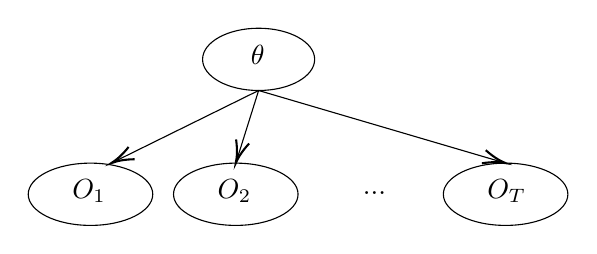
\begin{tikzpicture}[x=0.75pt,y=0.75pt,yscale=-1,xscale=1]
		%uncomment if require: \path (0,300); %set diagram left start at 0, and has height of 300
		
		%Straight Lines [id:da7972474226847348] 
		\draw    (221,85) -- (151.79,119.12) ;
		\draw [shift={(150,120)}, rotate = 333.76] [color={rgb, 255:red, 0; green, 0; blue, 0 }  ][line width=0.75]    (10.93,-3.29) .. controls (6.95,-1.4) and (3.31,-0.3) .. (0,0) .. controls (3.31,0.3) and (6.95,1.4) .. (10.93,3.29)   ;
		%Shape: Ellipse [id:dp0226909827079409] 
		\draw   (194,70) .. controls (194,61.72) and (206.09,55) .. (221,55) .. controls (235.91,55) and (248,61.72) .. (248,70) .. controls (248,78.28) and (235.91,85) .. (221,85) .. controls (206.09,85) and (194,78.28) .. (194,70) -- cycle ;
		%Shape: Ellipse [id:dp597261072710862] 
		\draw   (110,135) .. controls (110,126.72) and (123.43,120) .. (140,120) .. controls (156.57,120) and (170,126.72) .. (170,135) .. controls (170,143.28) and (156.57,150) .. (140,150) .. controls (123.43,150) and (110,143.28) .. (110,135) -- cycle ;
		%Shape: Ellipse [id:dp7674512782916287] 
		\draw   (180,135) .. controls (180,126.72) and (193.43,120) .. (210,120) .. controls (226.57,120) and (240,126.72) .. (240,135) .. controls (240,143.28) and (226.57,150) .. (210,150) .. controls (193.43,150) and (180,143.28) .. (180,135) -- cycle ;
		%Shape: Ellipse [id:dp1187894984379172] 
		\draw   (310,135) .. controls (310,126.72) and (323.43,120) .. (340,120) .. controls (356.57,120) and (370,126.72) .. (370,135) .. controls (370,143.28) and (356.57,150) .. (340,150) .. controls (323.43,150) and (310,143.28) .. (310,135) -- cycle ;
		%Straight Lines [id:da8417223805404801] 
		\draw    (221,85) -- (210.6,118.09) ;
		\draw [shift={(210,120)}, rotate = 287.45] [color={rgb, 255:red, 0; green, 0; blue, 0 }  ][line width=0.75]    (10.93,-3.29) .. controls (6.95,-1.4) and (3.31,-0.3) .. (0,0) .. controls (3.31,0.3) and (6.95,1.4) .. (10.93,3.29)   ;
		%Straight Lines [id:da2646651612364299] 
		\draw    (221,85) -- (338.08,119.44) ;
		\draw [shift={(340,120)}, rotate = 196.39] [color={rgb, 255:red, 0; green, 0; blue, 0 }  ][line width=0.75]    (10.93,-3.29) .. controls (6.95,-1.4) and (3.31,-0.3) .. (0,0) .. controls (3.31,0.3) and (6.95,1.4) .. (10.93,3.29)   ;
		
		% Text Node
		\draw (130,126.44) node [anchor=north west][inner sep=0.75pt]    {$O_{1}$};
		% Text Node
		\draw (216,62) node [anchor=north west][inner sep=0.75pt]   [align=left] {$\displaystyle \theta $};
		% Text Node
		\draw (200,126.44) node [anchor=north west][inner sep=0.75pt]    {$O_{2}$};
		% Text Node
		\draw (330,126.44) node [anchor=north west][inner sep=0.75pt]    {$O_{T}$};
		% Text Node
		\draw (270,132.4) node [anchor=north west][inner sep=0.75pt]    {$...$};
		
		
		\end{tikzpicture}
	\end{figure}

	
	\begin{remark}
		Parameters outside the plate are often omitted.
	\end{remark}
	
	\begin{example}[Nested Plate]
		
	\end{example}
	
	\begin{example}[Overlapping Plate]
		
	\end{example}
	
	\begin{example}[Collective Inference]
		
	\end{example}
	
	\begin{definition}
		A \textbf{plate dependency model} consists of a template variable $A(U_1, \cdots, U_k)$ and template parents $B_1(\textbf{U}_1), \cdots, B_m(\textbf{U}_m)$, where $\textbf{U}_k \subseteq \{U_1, \cdots, U_k\}$. The conditional probability distribution in this model is $P(A|B_1, \cdots, B_m)$.
	\end{definition}

	\begin{figure}[H]
		\caption{Plate dependency model}
		\centering
		\medbreak
		\label{fig:1.2.4.3}

		
		\tikzset{every picture/.style={line width=0.75pt}} %set default line width to 0.75pt        
		
		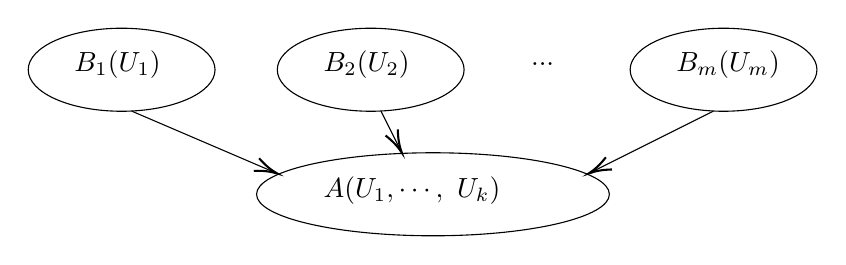
\begin{tikzpicture}[x=0.75pt,y=0.75pt,yscale=-1,xscale=1]
		%uncomment if require: \path (0,300); %set diagram left start at 0, and has height of 300
		
		%Shape: Ellipse [id:dp631765110353913] 
		\draw   (200,170) .. controls (200,158.95) and (238.06,150) .. (285,150) .. controls (331.94,150) and (370,158.95) .. (370,170) .. controls (370,181.05) and (331.94,190) .. (285,190) .. controls (238.06,190) and (200,181.05) .. (200,170) -- cycle ;
		%Shape: Ellipse [id:dp8739887854198307] 
		\draw   (90,110) .. controls (90,98.95) and (110.15,90) .. (135,90) .. controls (159.85,90) and (180,98.95) .. (180,110) .. controls (180,121.05) and (159.85,130) .. (135,130) .. controls (110.15,130) and (90,121.05) .. (90,110) -- cycle ;
		%Shape: Ellipse [id:dp7975375398256144] 
		\draw   (210,110) .. controls (210,98.95) and (230.15,90) .. (255,90) .. controls (279.85,90) and (300,98.95) .. (300,110) .. controls (300,121.05) and (279.85,130) .. (255,130) .. controls (230.15,130) and (210,121.05) .. (210,110) -- cycle ;
		%Shape: Ellipse [id:dp8634161057218073] 
		\draw   (380,110) .. controls (380,98.95) and (400.15,90) .. (425,90) .. controls (449.85,90) and (470,98.95) .. (470,110) .. controls (470,121.05) and (449.85,130) .. (425,130) .. controls (400.15,130) and (380,121.05) .. (380,110) -- cycle ;
		%Straight Lines [id:da6485499931155878] 
		\draw    (140,130) -- (208.16,159.21) ;
		\draw [shift={(210,160)}, rotate = 203.2] [color={rgb, 255:red, 0; green, 0; blue, 0 }  ][line width=0.75]    (10.93,-3.29) .. controls (6.95,-1.4) and (3.31,-0.3) .. (0,0) .. controls (3.31,0.3) and (6.95,1.4) .. (10.93,3.29)   ;
		%Straight Lines [id:da4286679970618126] 
		\draw    (260,130) -- (269.11,148.21) ;
		\draw [shift={(270,150)}, rotate = 243.43] [color={rgb, 255:red, 0; green, 0; blue, 0 }  ][line width=0.75]    (10.93,-3.29) .. controls (6.95,-1.4) and (3.31,-0.3) .. (0,0) .. controls (3.31,0.3) and (6.95,1.4) .. (10.93,3.29)   ;
		%Straight Lines [id:da1467286491940989] 
		\draw    (420,130) -- (361.79,159.11) ;
		\draw [shift={(360,160)}, rotate = 333.43] [color={rgb, 255:red, 0; green, 0; blue, 0 }  ][line width=0.75]    (10.93,-3.29) .. controls (6.95,-1.4) and (3.31,-0.3) .. (0,0) .. controls (3.31,0.3) and (6.95,1.4) .. (10.93,3.29)   ;
		
		% Text Node
		\draw (231,160.4) node [anchor=north west][inner sep=0.75pt]    {$A( U_{1} ,\cdots ,\ U_{k})$};
		% Text Node
		\draw (111,99.4) node [anchor=north west][inner sep=0.75pt]    {$B_{1}(\boldsymbol{U}_{1})$};
		% Text Node
		\draw (231,99.4) node [anchor=north west][inner sep=0.75pt]    {$B_{2}(\boldsymbol{U}_{2})$};
		% Text Node
		\draw (401,99.4) node [anchor=north west][inner sep=0.75pt]    {$B_{m}(\boldsymbol{U}_{m})$};
		% Text Node
		\draw (331,105.4) node [anchor=north west][inner sep=0.75pt]    {$...$};
		\end{tikzpicture}
	\end{figure}

	\begin{definition}
		The concrete instantiation (\textbf{ground network}) of a plate dependency model consists of instantiations $u_1, \cdots, u_k$ of $U_1, \cdots, U_k$.
	\end{definition}
	
	\subsection{Local Structures}
	\begin{definition}
		A \textbf{general conditional probability distribution} $P(X|Y_1, \cdots, Y_k)$ specifies distribution over $X$ for each realization of $Y_1, \cdots, Y_k$. Any factor $\phi$ with scope $\{X, Y_1, \cdots, Y_K\}$ satisfying
		\begin{align}
			\sum_x \phi(x, y_1, \cdots, y_k) = 1\quad \forall y_1, \cdots, y_k
		\end{align}
		defines a valid general CPD.
	\end{definition}
	
	\begin{definition}[Context-Specific Independence]
		Let $P \in \Delta(\mc{X})$, let $X, Y \in \mc{X}$ and $\textbf{Z}, \textbf{C} \subseteq \mc{X}$. Let $\textbf{c}$ be a realization of random variables $\textbf{C}$. Then $X$ is said to be independent from $Y$ given $Y$ in the context $c$, denoted as $(X \indep_c Y|\textbf{Z}, \textbf{c})$, if
		\begin{align}
			P(X, Y | \textbf{Z}, \textbf{c}) = P(X| \textbf{Z}, \textbf{c}) P(Y| \textbf{Z}, \textbf{c})
		\end{align}
	\end{definition}
	
	\subsection{Pairwise Markov Networks}
	\begin{definition}
		A \textbf{pairwise Markov network} is a undirected graph whose nodes are random variables $X_1, \cdots, X_n$ and each edge $(X_i, X_j)$ is associated with a factor $\phi_{ij}(X_i, X_j)$.
	\end{definition}

	\begin{figure}[H]
		\caption{A simple pairwise Markov network}
		\centering
		\medbreak
		\label{fig:1.3.1.1}
		\tikzset{every picture/.style={line width=0.75pt}} %set default line width to 0.75pt        
		
		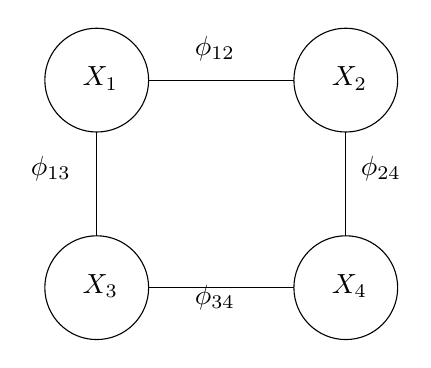
\begin{tikzpicture}[x=0.75pt,y=0.75pt,yscale=-1,xscale=1]
		%uncomment if require: \path (0,300); %set diagram left start at 0, and has height of 300
		
		%Shape: Circle [id:dp6148735435356301] 
		\draw   (100,145) .. controls (100,131.19) and (111.19,120) .. (125,120) .. controls (138.81,120) and (150,131.19) .. (150,145) .. controls (150,158.81) and (138.81,170) .. (125,170) .. controls (111.19,170) and (100,158.81) .. (100,145) -- cycle ;
		%Shape: Circle [id:dp7313274510409606] 
		\draw   (220,145) .. controls (220,131.19) and (231.19,120) .. (245,120) .. controls (258.81,120) and (270,131.19) .. (270,145) .. controls (270,158.81) and (258.81,170) .. (245,170) .. controls (231.19,170) and (220,158.81) .. (220,145) -- cycle ;
		%Shape: Circle [id:dp44334149215305474] 
		\draw   (100,245) .. controls (100,231.19) and (111.19,220) .. (125,220) .. controls (138.81,220) and (150,231.19) .. (150,245) .. controls (150,258.81) and (138.81,270) .. (125,270) .. controls (111.19,270) and (100,258.81) .. (100,245) -- cycle ;
		%Shape: Circle [id:dp9337154446683626] 
		\draw   (220,245) .. controls (220,231.19) and (231.19,220) .. (245,220) .. controls (258.81,220) and (270,231.19) .. (270,245) .. controls (270,258.81) and (258.81,270) .. (245,270) .. controls (231.19,270) and (220,258.81) .. (220,245) -- cycle ;
		%Straight Lines [id:da08957161211937148] 
		\draw    (125,170) -- (125,220) ;
		%Straight Lines [id:da24893313190023614] 
		\draw    (150,145) -- (220,145) ;
		%Straight Lines [id:da9153218821089248] 
		\draw    (245,170) -- (245,220) ;
		%Straight Lines [id:da2667760341360965] 
		\draw    (150,245) -- (220,245) ;
		
		% Text Node
		\draw (117,137.4) node [anchor=north west][inner sep=0.75pt]    {$X_{1}$};
		% Text Node
		\draw (237,137.4) node [anchor=north west][inner sep=0.75pt]    {$X_{2}$};
		% Text Node
		\draw (117,237.4) node [anchor=north west][inner sep=0.75pt]    {$X_{3}$};
		% Text Node
		\draw (237,237.4) node [anchor=north west][inner sep=0.75pt]    {$X_{4}$};
		% Text Node
		\draw (92,180.4) node [anchor=north west][inner sep=0.75pt]    {$\phi _{13}$};
		% Text Node
		\draw (171,122.4) node [anchor=north west][inner sep=0.75pt]    {$\phi _{12}$};
		% Text Node
		\draw (251,180.4) node [anchor=north west][inner sep=0.75pt]    {$\phi _{24}$};
		% Text Node
		\draw (171,242.4) node [anchor=north west][inner sep=0.75pt]    {$\phi _{34}$};
		
		
		\end{tikzpicture}
	\end{figure}
	
	\subsection{General Gibbs Distributions}
	\begin{definition}
		A \textbf{Gibbs distribution} over random variables $X_1, \cdots, X_n$ is specified by a set of general factors, $\Phi = \{\phi_i(D_i)\}_{i=1}^k$, where each $D_i \subseteq \{X_1, \cdots, X_n\}$. The corresponding unnormalized probability and partition function are
		\begin{align}
			\tilde{P}_\Phi(X_1, \cdots, X_n) = \prod_{i=1}^k \phi_i(D_i) \\
			Z_\Phi = \sum_{X_1, \cdots, X_n} \tilde{P}_\Phi(X_1, \cdots, X_n)
		\end{align}
		The probability distribution is
		\begin{align}
			P_\Phi(X_1, \cdots, X_n) = \frac{\tilde{P}_\Phi(X_1, \cdots, X_n)}{Z_\Phi}
		\end{align}
	\end{definition}
	
	\begin{definition}
		The \textbf{induced Markov network} of a set of factors $\Phi = \{\phi_i(D_i)\}_{i=1}^k$, where $D_i \subseteq \{X_1, \cdots, X_n\}$, denoted as $H_\Phi$, is a network in which there is an edge between $X_i$ and $X_j$ whenever $\exists\ m \in [k] \ s.t.\ X_i, X_j \in D_m$.
	\end{definition}
	
	\begin{definition}
		A probability distribution $P$ \textbf{factorizes} over a Markov network $H$ if there exists $\Phi = \{\phi_1(D_1), \cdots, \phi_k(D_k)\}$ such that $P = P_\Phi$ and $H = H_\Phi$.
	\end{definition}
	
	\begin{remark}
		There can be multiple factorizations of a given Markov network.
	\end{remark}
	
	\begin{definition}
		A trail (path) $X_1 - \cdots - X_n$ in a Markov network is \textbf{active} given a set of nodes \textbf{Z} if no $X_i$ is in \textbf{Z}.
	\end{definition}

	\subsection{Conditional Random Fields}
	\begin{definition}[CRF]
		A \textbf{CRF representation} over random variables $X \cup Y$ consists of a set of factors $\Phi = \{\phi_1(D_1), \cdots, \phi_k(D_k)\}$, where $D_i \subseteq X \cup Y$.
		
		The unnormalized probability and partition function are defined as
		\begin{align}
			\tilde{P}(X, Y) = \prod_{i=1}^k \phi_i(D_i) \\
			Z(X) = \sum_Y \tilde{P}(X, Y)
		\end{align}
		The conditional probability is therefore
		\begin{align}
			P(Y|X) = \frac{1}{Z(X)} \tilde{P}(X, Y)
		\end{align}
	\end{definition}
	
	\begin{remark}
		A CRF is parameterized the same as a Gibbs distribution, both of them are defined using factors. However, they are normalized differently, the partition function in CRF, $Z(X)$, depends on the particular realization of $X$, but $Z_\Phi$ depends on factors only.
	\end{remark}
	
	\begin{example}[Logistic model as a CRF]
		Let $X_1, \cdots, X_k$ denote the $k$ random variables serve as features to generate the target variable $Y$. Figure \ref{fig:1.3.3.1} illustrates the logistic model as a Bayesian network. For simplicity, assume $X_i$ and $Y$ are all binary. Define factors
		\begin{align}
			\phi_i(X_i, Y) := \exp(w_i \id{X_i=1 \land Y=1}) = \exp(w_i X_i Y)
		\end{align}
		Therefore, the unnormalized probabilities are
		\begin{align}
			\tilde{P}(Y=0, X_i) &= \prod_{i=1}^k \exp(w_i X_i 0) = 1 \\
			\tilde{P}(Y=1, X_i) &= \prod_{i=1}^k \exp(w_i X_i) = \exp \left(\sum_{i=1}^k w_i X_i\right)
		\end{align}
		Then, the CPD can be expressed as
		\begin{align}
			P(Y=1|X_1, \cdots, X_k) &= \frac{\tilde{P}(Y=1, X_i)}{\tilde{P}(Y=0, X_i) + \tilde{P}(Y=1, X_i)} \\
			&= \frac{\exp \left(\sum_{i=1}^k w_i X_i\right)}{1 + \exp \left(\sum_{i=1}^k w_i X_i\right)} \\
			&= \frac{1}{1 + \exp \left(-\sum_{i=1}^k w_i X_i\right)} = \sigma \left(\sum_{i=1}^k w_i X_i\right)
		\end{align}
	\end{example}

	\begin{figure}[H]
		\caption{Logistic model as a Bayesian network}
		\centering
		\medbreak
		\label{fig:1.3.3.1}
		\tikzset{every picture/.style={line width=0.75pt}} %set default line width to 0.75pt        
		
		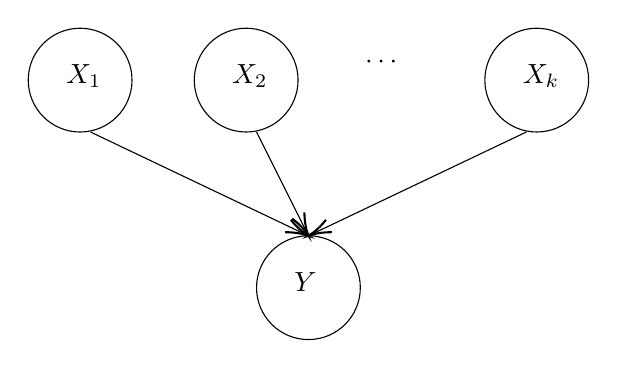
\begin{tikzpicture}[x=0.75pt,y=0.75pt,yscale=-1,xscale=1]
		%uncomment if require: \path (0,300); %set diagram left start at 0, and has height of 300
		
		%Shape: Circle [id:dp12532593899895228] 
		\draw   (130,55) .. controls (130,41.19) and (141.19,30) .. (155,30) .. controls (168.81,30) and (180,41.19) .. (180,55) .. controls (180,68.81) and (168.81,80) .. (155,80) .. controls (141.19,80) and (130,68.81) .. (130,55) -- cycle ;
		%Shape: Circle [id:dp2762283424913996] 
		\draw   (210,55) .. controls (210,41.19) and (221.19,30) .. (235,30) .. controls (248.81,30) and (260,41.19) .. (260,55) .. controls (260,68.81) and (248.81,80) .. (235,80) .. controls (221.19,80) and (210,68.81) .. (210,55) -- cycle ;
		%Shape: Circle [id:dp8409084819168187] 
		\draw   (350,55) .. controls (350,41.19) and (361.19,30) .. (375,30) .. controls (388.81,30) and (400,41.19) .. (400,55) .. controls (400,68.81) and (388.81,80) .. (375,80) .. controls (361.19,80) and (350,68.81) .. (350,55) -- cycle ;
		%Shape: Circle [id:dp8580515955485923] 
		\draw   (240,155) .. controls (240,141.19) and (251.19,130) .. (265,130) .. controls (278.81,130) and (290,141.19) .. (290,155) .. controls (290,168.81) and (278.81,180) .. (265,180) .. controls (251.19,180) and (240,168.81) .. (240,155) -- cycle ;
		%Straight Lines [id:da6449546534492006] 
		\draw    (160,80) -- (263.19,129.14) ;
		\draw [shift={(265,130)}, rotate = 205.46] [color={rgb, 255:red, 0; green, 0; blue, 0 }  ][line width=0.75]    (10.93,-3.29) .. controls (6.95,-1.4) and (3.31,-0.3) .. (0,0) .. controls (3.31,0.3) and (6.95,1.4) .. (10.93,3.29)   ;
		%Straight Lines [id:da5935723910459691] 
		\draw    (240,80) -- (264.11,128.21) ;
		\draw [shift={(265,130)}, rotate = 243.43] [color={rgb, 255:red, 0; green, 0; blue, 0 }  ][line width=0.75]    (10.93,-3.29) .. controls (6.95,-1.4) and (3.31,-0.3) .. (0,0) .. controls (3.31,0.3) and (6.95,1.4) .. (10.93,3.29)   ;
		%Straight Lines [id:da2293241975385838] 
		\draw    (370,80) -- (266.81,129.14) ;
		\draw [shift={(265,130)}, rotate = 334.53999999999996] [color={rgb, 255:red, 0; green, 0; blue, 0 }  ][line width=0.75]    (10.93,-3.29) .. controls (6.95,-1.4) and (3.31,-0.3) .. (0,0) .. controls (3.31,0.3) and (6.95,1.4) .. (10.93,3.29)   ;
		
		% Text Node
		\draw (147,46.32) node [anchor=north west][inner sep=0.75pt]    {$X_{1}$};
		% Text Node
		\draw (227,46.32) node [anchor=north west][inner sep=0.75pt]    {$X_{2}$};
		% Text Node
		\draw (367,46.32) node [anchor=north west][inner sep=0.75pt]    {$X_{k}$};
		% Text Node
		\draw (291,42.4) node [anchor=north west][inner sep=0.75pt]    {$\cdots $};
		% Text Node
		\draw (257,146.32) node [anchor=north west][inner sep=0.75pt]    {$Y$};
		
		
		\end{tikzpicture}
	\end{figure}

	\subsection{Independencies in Markov Networks}
	\begin{definition}
		Two nodes $X$ and $Y$ in a Markov network $H$ are \textbf{separated} given set of nodes $Z$ if there is no active trail (path) in $H$ between $X$ and $Y$ given $Z$. Denoted as $\sep_H(X, Y|Z)$
	\end{definition}
	
	\begin{theorem}
		If distribution $P$ factorizes over Markov network $H$, then $P$ satisfies
		\begin{align}
			\sep_H(X, Y|Z) \implies X \indep Y | Z
		\end{align} 
	\end{theorem}
	
	\begin{proof}
		
	\end{proof}
	
	\begin{definition}
		Let $I(H)$ denote the collection of independencies induced by $H$:
		\begin{align}
			\mc{I}(H) := \{(X \indep Y | Z: \sep_H(X, Y | Z)\}
		\end{align}
		If $P$ satisfies $\mc{I}(H)$, then $H$ is an \textbf{independency map} (I-map) of $P$.
	\end{definition}
	
	\begin{theorem}
		If $P$ factorizes over $H$, then $H$ is an I-map of $P$.
	\end{theorem}
	
	\begin{proof}
		
	\end{proof}
	
	\begin{theorem}[Hammersley Clifford]
		For a \ul{positive} distribution $P$ (i.e., $P(x) >0$ for all $x$), if $H$ is an I-map for $P$, then $P$ factorizes over $H$.
	\end{theorem}
	
	\begin{proof}
		
	\end{proof}


	\section{Inference}
	\section{Learning}
	\subsection{Learning Network Structure}
	\paragraph{Motivation} We have discussed methods to estimate parameters given a network structure and dataset, however, ways to choose the structure remains uncovered.
	Specifically, given a dataset $D$, we have to choose one graph $G$ as the skeleton of our model.

	 Compared with the graph representing the true data generating process, if the specified graph $G$ contains less edges, $G$ imposes more independence assumptions than necessary.
	 In contrast, if the specified graph $G$ has extra edges, then the redundant dependencies would require more parameters to be fitted using the limited dataset and leads to bad generalization.
	
	To select the best structure $G$ given dataset $D$, we can define a \textbf{scoring function} taking both $G$ and $D$ as arguments.
	Then the model selection problem turns into an optimization problem:
	\begin{align}
		\tx{Optimal } G^* := \argmax_{G \in \tx{all models}} \tx{score}(G, D)
	\end{align}

	\subsubsection{Likelihood Structure Scores}
	\begin{definition}
		\textbf{Likelihood structure score} defines the compatibleness between a graph $G$ and dataset $D$ as
		\begin{align}
			\tx{score}_L (G; D) := \ell(G_{\hat{\theta}}; D)
		\end{align}
		Where $\hat{\theta}$ is the maximum likelihood estimations from of parameters in graph $G$ from dataset $D$, and $\ell$ is the log-likelihood function.
	\end{definition}
\end{document}





















